% CSCI-B 565 Assignment 1 by Supreeth Keragodu Suryaprakash, Hanfei Mei and Ishtiak Zaman
\documentclass{article}

\newtheorem{thm}{Theorem}

% Set left margin - The default is 1 inch, so the following 
% command sets a 1.25-inch left margin.
\setlength{\oddsidemargin}{0.25in}

% Set width of the text - What is left will be the right margin.
% In this case, right margin is 8.5in - 1.25in - 6in = 1.25in.
\setlength{\textwidth}{6in}

% Set top margin - The default is 1 inch, so the following 
% command sets a 0.75-inch top margin.
\setlength{\topmargin}{-0.25in}

% Set height of the header
\setlength{\headheight}{0.3in}

% Set vertical distance between the header and the text
\setlength{\headsep}{0.2in}

% Set height of the text
\setlength{\textheight}{9in}

% Set vertical distance between the text and the
% bottom of footer
\setlength{\footskip}{0.1in}

% Set the beginning of a LaTeX document
\usepackage{tikz}
\usepackage{multirow}
\usepackage{fullpage}
\usepackage{graphicx}
\usepackage{amsthm}
\usepackage{amssymb}
\usepackage{algpseudocode}
\usepackage{amsmath}
\usepackage{tabularx}
\graphicspath{ {Images/} }
%%%%%%%%%%%%%%%%%%%%%%%%%%%%%

\begin{document}\title{CSCI-B 657: Computer Vision \\ Assignment 2 : Image Warping, Matching and Stiching \\ Final Report}         % Enter your title between curly braces
	\author{Ishtiak Zaman (izaman@indiana.edu) \\ Hanfei Mei (hanfei@indiana.edu) \\Supreeth Keragodu Suryaprakash(skeragod@indiana.edu)}        % Enter your name between curly braces
	% Enter your name between curly braces
	\date{\today}          % Enter your date or \today between curly braces
	\maketitle
	
	\makeatother
	
	\pagestyle{plain}
		\part{Image Matching}
	
	\section{Explanation and Results: }
	
	\begin{enumerate}
		\item
		
		The solution for this has been implemented in \textbf{\textit{SIFT\_match}} function. \\
		\textit{\textbf{Input:} source image, query image, threshold value 1, threshold value 2. \\
		\textbf{Output:} Returns the number of matching points.}
	
		\textbf{Implementation}:
		\begin{enumerate}
			\item We are finding the sift descriptor vectors for both the images.
			\item  For each pair of \textit{(s\_d, q\_d)}, \textit{s\_d} is a sift descriptor in source image and \textit{q\_d} is a sift descriptor in query image. We'll compute the Euclidean distance for both.
		\item  For each s\_d in query image, We'll find the best two matching pairs of \textit{(s\_d, q\_d)}, compute radio by \textit{closest\_distance\textit{(s\_d,q\_d1)}/second\_closest\_distance\textit{(s\_d,q\_d2)}}.
		\item If ratio is less than the threshold, it is regarded as a pair of match points, draw a line in the merged image and return the total number of matched points.
		\end{enumerate}
		
		\textbf{Output Image:}
		
		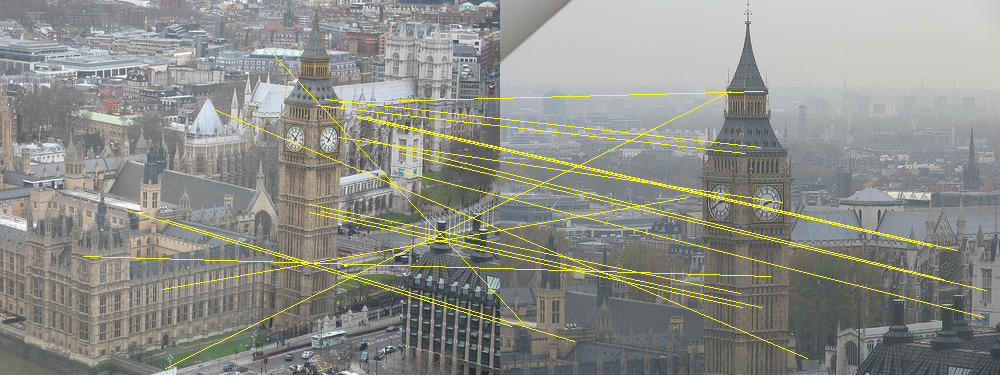
\includegraphics[height=6cm,width=16cm]{1}
		\begin{center}
			\textit{	(Fig 1 : Matching points for bigben\_2.jpg and bigben\_3.jpg)}
		\end{center}
	
		
		\textbf{How to Run?}
		
		Command Line : \textit{./a2 part1 $<img1.extension>  <img1.extension>$}
		
		This will provide you with three options, press 1 and hit enter.
		
		
		\item 
		
		
		 The solution has been implemented in the \textit{maximum\_key\_points} function. 
		 
		\textbf{Input :} argument\_count, argument\_vector, an interger value to  provide solution for which problem. 
		
		\textbf{Output :} Prints the result on the console.
		
	\textbf{Implementation :} 
	We are making use of the function that was explained in the previous question. The output would be the total number of key points matched. We have used a $<string, interger>$ vector to store the total number of match points for each query image with the source image. In the string part of the pair we are storing the file name of the query images. We are then sorting the vector based on $2^{nd}$ field (which contains integer values) and are displaying the result.
		
			\textbf{How to Run?}
			
			Command Line : \textit{./a2 part1 $<img1.extension>  <img1.extension> ... $}
			
			This will provide you with three options, press 2 and hit enter.
				
				\begin{center}
					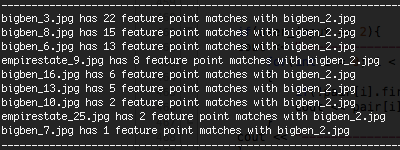
\includegraphics[height=3cm,width=7cm]{2} \\
					\textit{	(Fig 2 : Sorted the vector in the increasing order of matched key points wrt source image.)}
				\end{center}
			
			\item 
			
			The solution for this question has been implemented in \textit{maximum\_key\_points} function
			
			\textbf{Input :} argument\_count, argument\_vector, an interger value to  provide solution for which problem. 
			
			\textbf{Output :} Prints the result on the console.
			
			\textbf{Implementation :} We will be calculating the matching points in the function that was explained in question 1. The solution to this question has only change one from the previous question i.e. We will be running the source image against all the 100 images provided in part1\_images folder provided by the Professor. We are storing the values in a vector as explained in the previous question and are sorting it in the same fashion. We will pick the top 10 images from the vector. We will caculate the number of correct predictions and the wrong predictions for 10, thereby calculating the precision factor. Formula to find the precision is as below,
				\begin{center}
					
			
			
			\fbox{\begin{minipage}{30em}
					\begin{center}
						
							P = $\dfrac{correct\_prediction}{correct\_prediction + wrong\_prediction} * 100$
						
					\end{center}
				\end{minipage}} \\
					\end{center}
					
					
					
						\begin{center}
							\begin{tabular}{||c c c ||} 
								\hline
								Serial Number & File Name & Precision \\ [0.5ex] 
								\hline\hline
								1 & bigben\_2.jpg& 60\% \\ 
								\hline
								2 & colosseum\_11.jpg & 30\% \\
								\hline
								3 & eiffel\_1.jpg	& 20\%  \\
								\hline
								4 & empirestate\_10 & 50\%  \\
								\hline
								5 & londoneye\_12.jpg &   30\%\\ 
								\hline
								6 & louvre\_10.jpg	 & 20\%  \\
								\hline
								7 & notredame\_1.jpg & 30\%  \\
								\hline
								8 & sanmarco\_1 &30\%  \\
								\hline
								9 & tatemodern\_11.jpg & 10\%  \\
								\hline
								10 & trafalgarsquare\_1.jpg & 50\% \\
								\hline
							\end{tabular}
						\end{center}
						
							\textbf{How to Run?}
							
							Command Line : \textit{./a2 part1 $<img1.extension>  <img1.extension> ... $}
							
							e.g. \textit{./a2 part1 part1\_images/louvre\_10.jpg  part1\_images/*.jpg}
							
							This will provide you with three options, press 3 and hit enter. You can view the number of keypoints matched with each image on the console as well as the top 10 matched images and the precision value.
							
							\begin{center}
								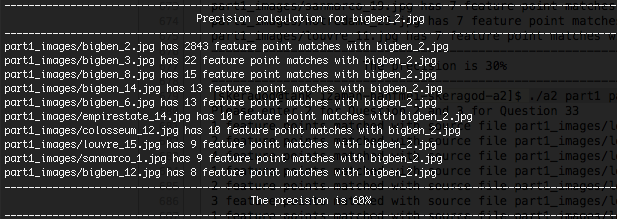
\includegraphics[height=3cm,width=7cm]{3} \\
								\textit{	(Fig 3 : Output screengrab for Bigben\_2.jpg which has a precision of 60\%)}
							\end{center}
							
				
				\item 
				The solution for this has been implemented in \textbf{\textit{SIFT\_summary\_match}} function. \\
				\textbf{Input:} Source Image, Query Image, k, w. \\
				\textbf{output:} Number of match points in both the images. \\
				\textbf{Implementation:} 
					\begin{enumerate}
				\item We have used gaussian random to generate k summary vectors. Each vector contains 128 random number which obeys the 0,1 Guassian Distribution.
				\item Calculate k features $f(v)$ for each descriptor in both source image and query image.
			\item For each descriptor d in source image, find a few candidates in query Image which has a similar $f(v)$ with $f(d)$.
				\item For every descriptor in source image, find the first and second closest descriptors in candidates.
			\item Compute the ratio of the most and second similar candidate descriptor for each descriptor $d$ and if the ratio is less than the threshold, it is regarded as a match point for $d$.
				\end{enumerate}
				
				\textbf{Running time:} it works a little faster than the normal function. A random 50 iterations in \textit{SIFT\_match} will take $68.349s$ and \textit{SIFT\_summary\_match} will take $67.251s$ because of the dimensionality reduction.		
				
										
		\begin{center}
			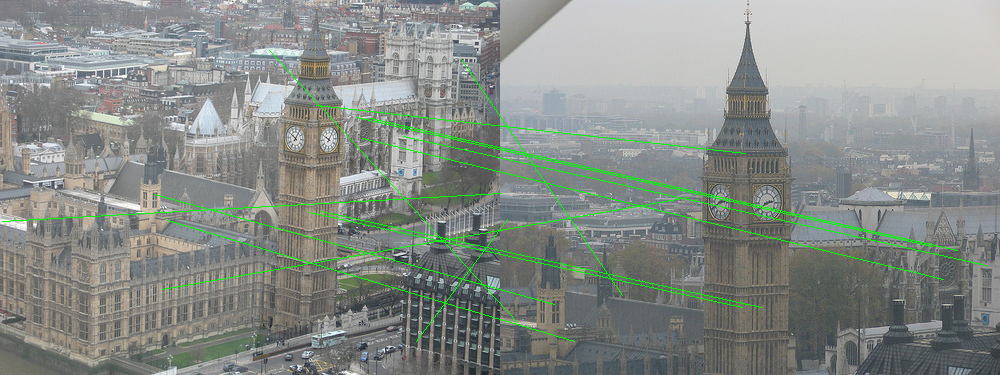
\includegraphics[height=6cm,width=16cm]{3a} \\
			\textit{	(Fig 4: Output of the SIFT\_summary\_match function for bigben\_2.jpg and bigben\_3.jpg )}
		\end{center}
		
	\end{enumerate}
		
	
			\part{ Image Warping and Homographies}	
			\begin{enumerate}
				\item  \textbf{Transformation:}
						We used inverse warping to get a projection of an image given a 3x3 transformation matrix. During the inverse warping method, when some pixel in the destination image points to a pixel outside of the source image dimensions, we used black pixel for those missing parts. When we need to get a non-integer pixel value from the source image, we used nearest neighbor interpolation. 
						
						Following is an example of transformation of the left image into the right one using the transformation matrix $[[0.907,0.258,-182],[-0.153,1.44,58],[-0.000306,0.000731,1]]$. The black area on the right image does not have any correspondences with any part of the source image.
						
								\begin{center}
									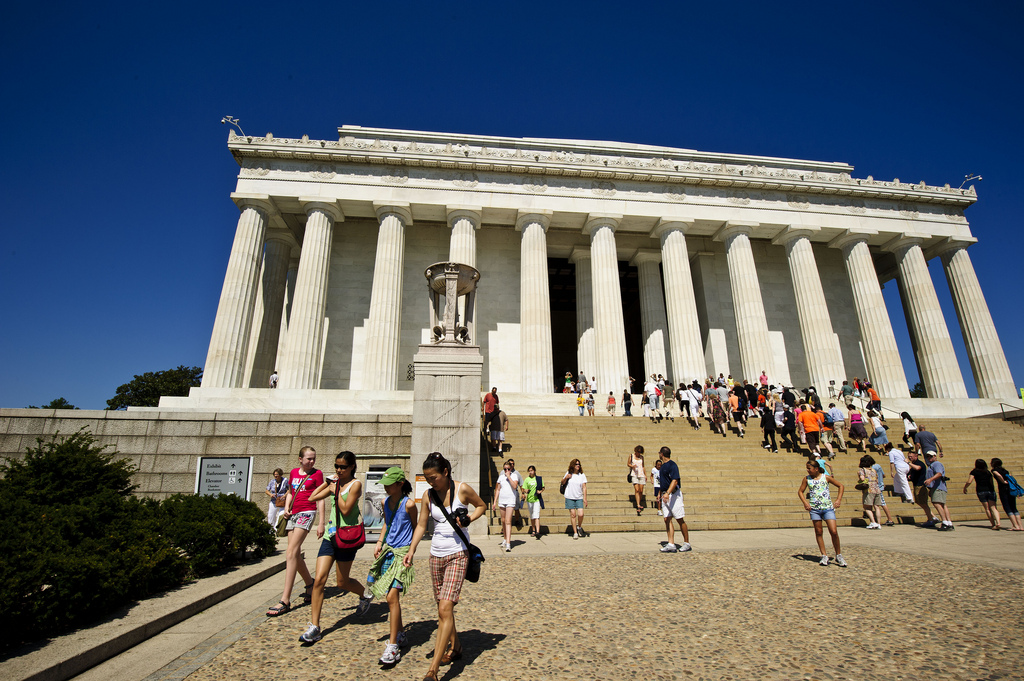
\includegraphics[height=4cm,width=7.5cm]{21} 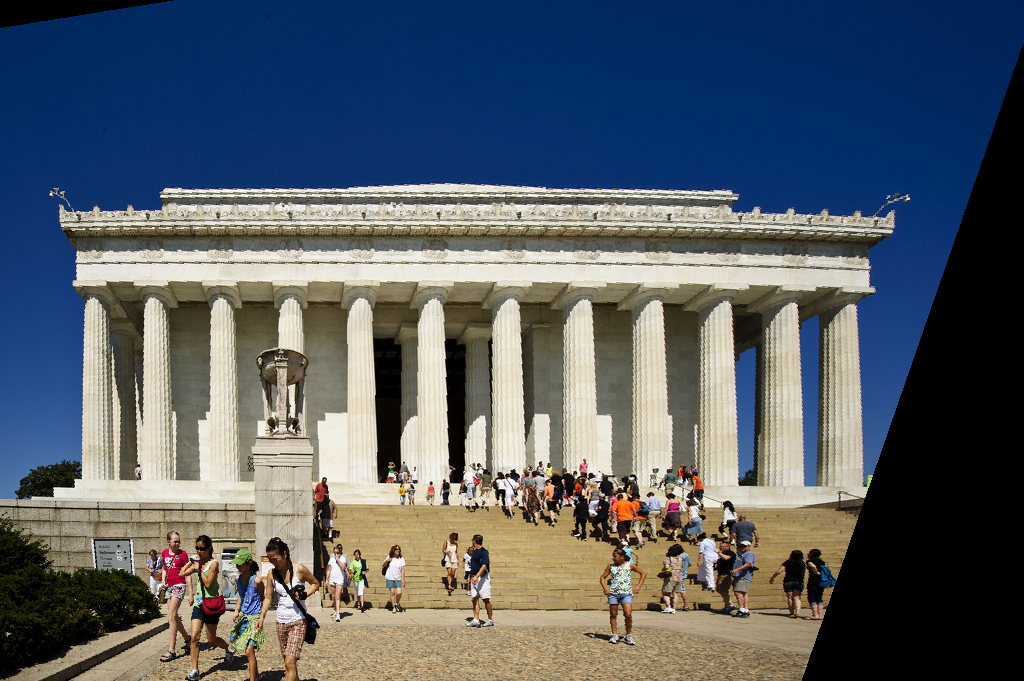
\includegraphics[height=4cm,width=7.5cm]{212} 
									\textit{	(Fig 5: Depiction of Tranformation )}
								\end{center}
								
					\item \textbf{Homography Estimation using RANSAC:}
					
					We used feature based alignment to get matches between two images using SIFT library. After getting the matches, we used RANSAC algorithm to maximize our inliers. In the RANSAC, we randomly choose 4 set of matches, get the transformation matrix by solving 8 equations with 8 unknown. 
					
					We used CImg linear solver library to do this task. Afterwards, we applied the transformation and see how many other matches agree with this transformation. We fine tuned our threshold parameters to maximize inliers with minimum false positive. The transformation with highest ratio of inliers is the winning hypothesis and we take that transformation to warp the second image. When the SIFT matches are good, we get a very good inlier ratio that results in a good warping of the image. But when the images are not very similar and the SIFT matches are not very good, we get a poor performance in the RANSAC with a low number of inlier matches. It results in a poor warped image. The performance of the RANSAC heavily depends on the quality of the SIFT matches. 
					
					Here are a few examples where the second image was warped into the third image in a way such that it looks like the second image was taken from the camera position of the first image.
					
					\begin{center}
						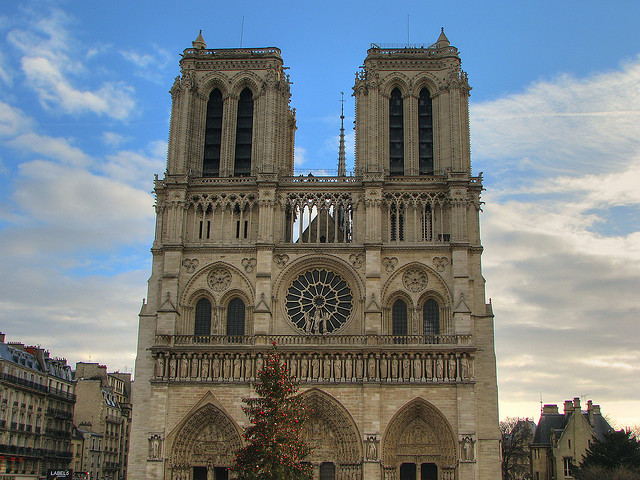
\includegraphics[height=4cm,width=5cm]{111a} 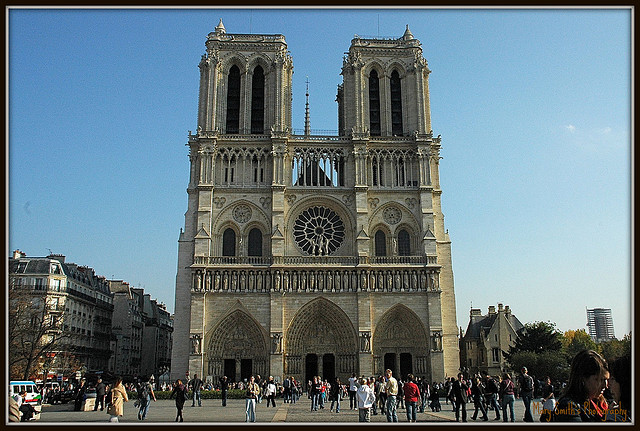
\includegraphics[height=4cm,width=5cm]{111b} 
						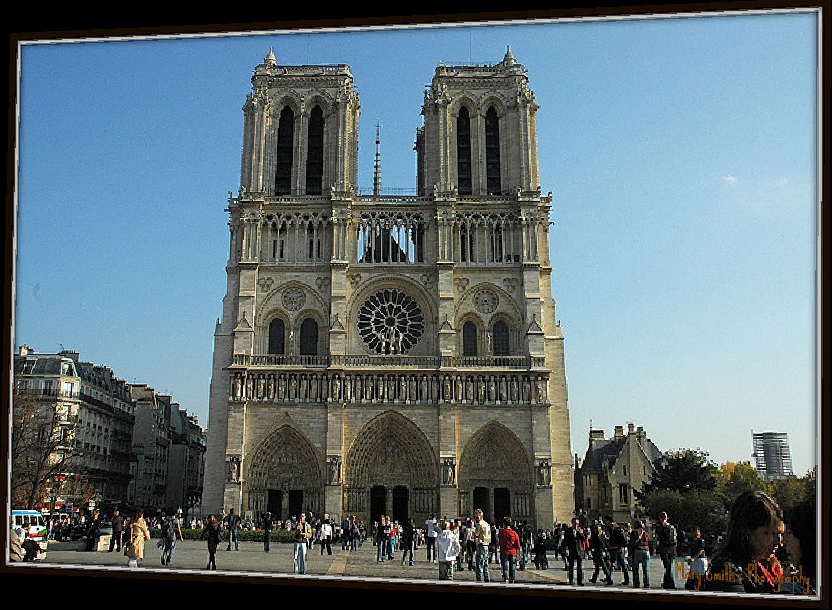
\includegraphics[height=4cm,width=5cm]{111c} 
					\end{center}
					
						\begin{center}
							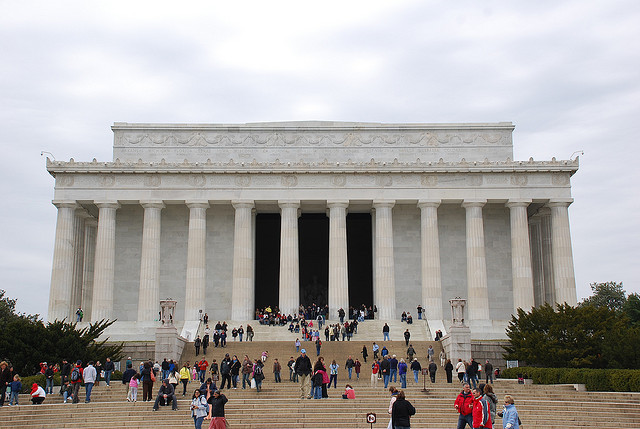
\includegraphics[height=4cm,width=5cm]{222a} 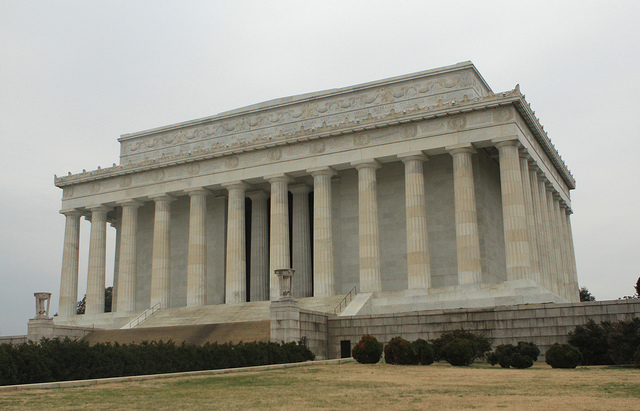
\includegraphics[height=4cm,width=5cm]{222b} 
							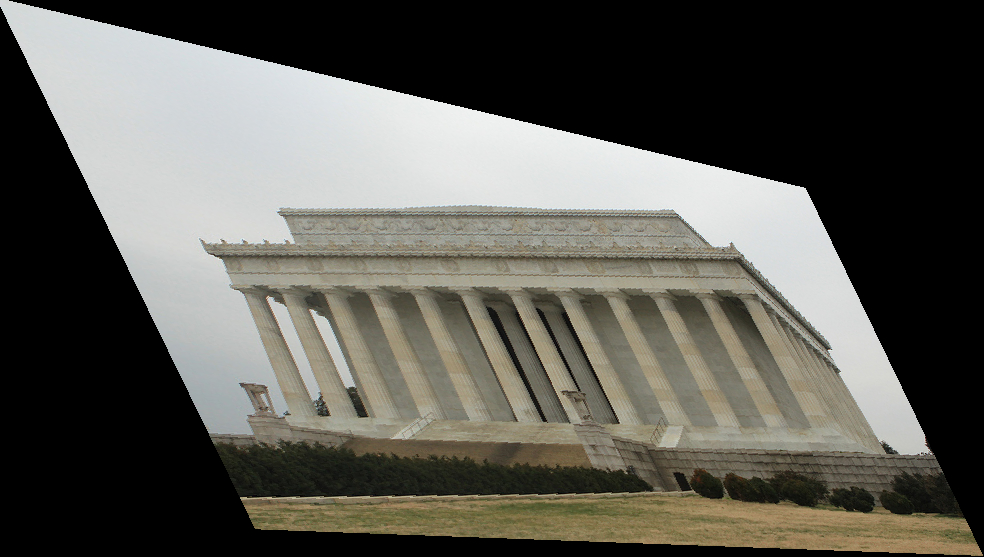
\includegraphics[height=4cm,width=5cm]{222c} 
						\end{center}
					
				\item \textit{Image Stitching:}
				After finding the homography transformation between two images, we used this information to make a panorama image by stitching the images together. We warped the second image as if it was taken from the camera position of the first image, and stitches the images together. There are common parts for both the two images, in those places we used mean blending technique to blend the pixels. 
				
				Here are some examples where we have stitched the first and second images to create the third panoramic image.
				
				\textbf{Examples :} 
				\begin{center}
					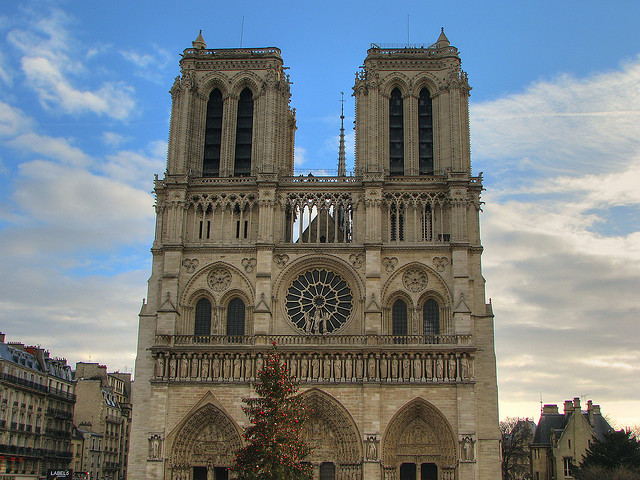
\includegraphics[height=7cm,width=7.5cm]{333a} 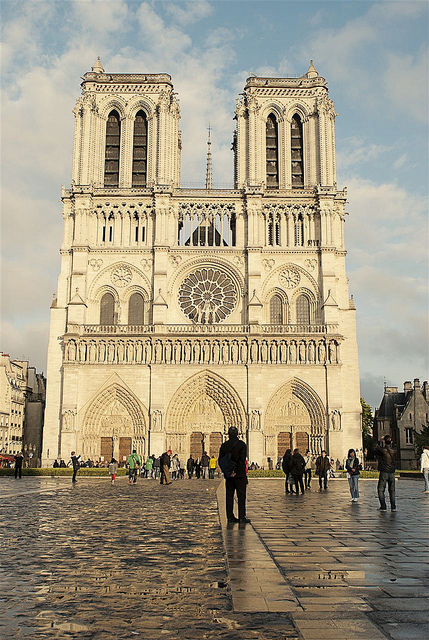
\includegraphics[height=7cm,width=7.5cm]{333b} 
					\textit{	(Fig 6a: Two images taken from different angles )} \\
					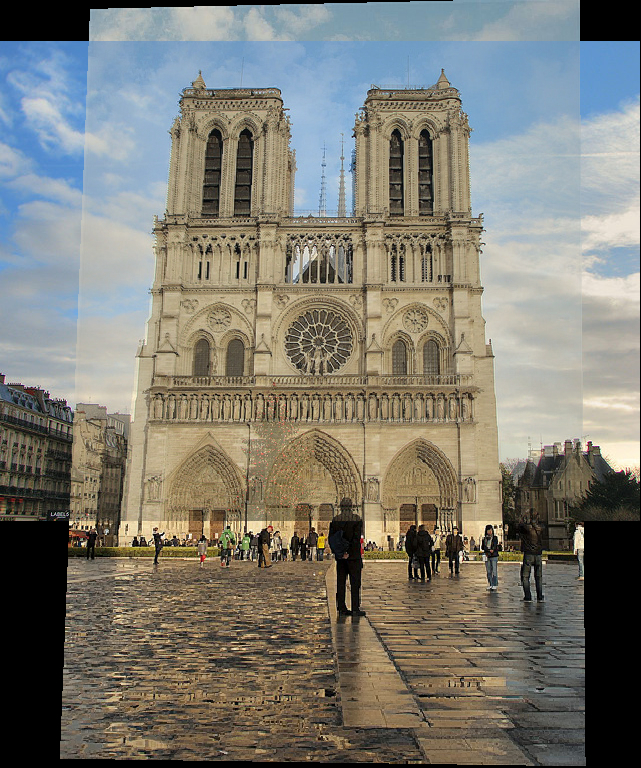
\includegraphics[height=7cm,width=7cm]{333c}  \\
					\textit{	(Fig 6b: Stiched Image )}
				\end{center}
				\begin{center}
					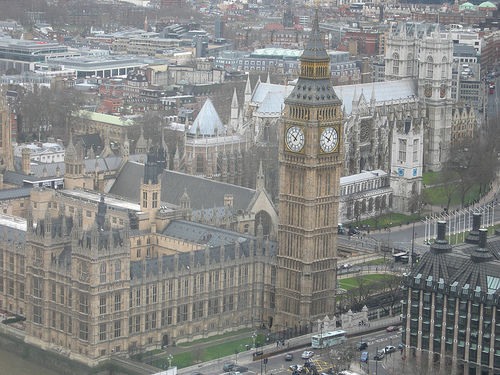
\includegraphics[height=7cm,width=7.5cm]{444a} 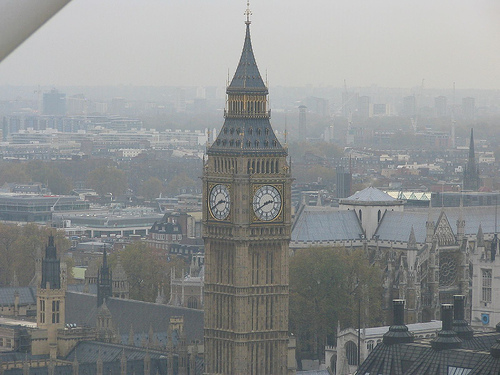
\includegraphics[height=7cm,width=7.5cm]{444b} 
					\textit{	(Fig 7a: Two images taken from different angles. Fig 7b: Stiched Image(below) )} \\
					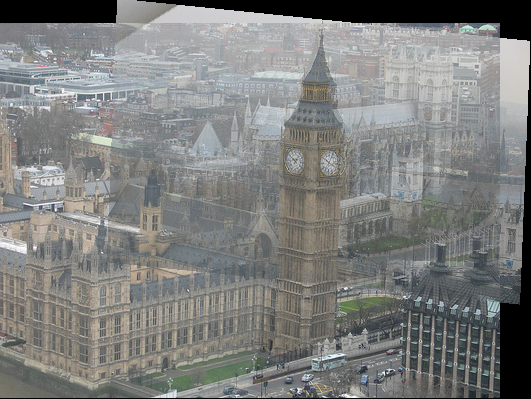
\includegraphics[height=7cm,width=7cm]{444c}  \\
				\end{center}
					
			\end{enumerate}
			
			\section{References :}
			\begin{itemize}
				\item http://www.cnblogs.com/yeahgis/archive/2012/07/13/2590485.html 
				\item Lecture slides by Prof. David Crandall
			\end{itemize}
		\end{document}